\documentclass[11pt,a4paper]{article}

\usepackage[T1]{fontenc}
\usepackage[utf8]{inputenc}
\usepackage{lmodern}
\usepackage{microtype}
\usepackage[margin=2.4cm]{geometry}
\usepackage{amsmath,amssymb,mathtools,bm}
\usepackage{graphicx}
\usepackage{booktabs,array,tabularx,multirow}
\usepackage[table]{xcolor}
\usepackage{caption}
\usepackage{enumitem}
\usepackage{float}
\usepackage[section]{placeins}
\usepackage{siunitx}
\usepackage[most]{tcolorbox}
\usepackage{tikz}
\usetikzlibrary{arrows.meta,positioning,decorations.pathmorphing,patterns,calc,fit}
\usepackage[colorlinks=true,linkcolor=blue!50!black,citecolor=green!40!black,urlcolor=blue!50!black]{hyperref}

\graphicspath{{../figures/}}
\captionsetup{font=small,labelfont=bf,margin=0.5cm}
\setlist{itemsep=2pt,topsep=4pt}
\setlength{\parskip}{3pt}
\renewcommand{\topfraction}{0.9}\renewcommand{\bottomfraction}{0.8}\renewcommand{\textfraction}{0.08}\renewcommand{\floatpagefraction}{0.8}

\newcommand{\Kbar}{\bar{K}}
\newcommand{\kb}{\bar{k}}
\newcommand{\qd}{q_{\mathrm{d}}}
\newcommand{\dqd}{\dot{q}_{\mathrm{d}}}
\newcommand{\phat}{\hat{p}_{\mathrm{o}}}
\newcommand{\T}{^{\top}}
\newcommand{\ke}{k_{\mathrm{e}}}
\newcommand{\kx}{k_{x}}
\newcommand{\Fdes}{F_{\mathrm{des}}}
\newcommand{\vapp}{v_{\mathrm{app}}}

\tcbset{summarybox/.style={colback=blue!3,colframe=blue!45!black,fonttitle=\bfseries,boxrule=0.6pt,arc=2pt,left=6pt,right=6pt,top=4pt,bottom=4pt}}

\hypersetup{pdftitle={Variable-Impedance Model Predictive Interaction Control for a 2-Link Planar Robot},pdfauthor={J. Zeynalli}}

\begin{document}

\begin{center}
{\LARGE Variable-Impedance Model Predictive Interaction Control\\[2pt] for a 2-Link Planar Robot}\\[8pt]
{\large Method, evaluation against classical MPIC, improvements and results}\\[12pt]
J.~Zeynalli\\[2pt]
{\small FAU Erlangen-N\"urnberg, Chair of Automatic Control}\\[2pt]
{\small Technical report, 2 November 2026 \;\textbullet\; repository \texttt{MPIC-2link-robot}, branches \texttt{vi-mpic} and \texttt{vi-mpic-v2}}
\end{center}

\begin{tcolorbox}[summarybox,title=Summary]
\begin{itemize}[leftmargin=12pt]
\item \textbf{Proposed.} Variable-impedance MPIC (VI-MPIC): the MPC plans the reference of a joint PD
  \emph{and} its Cartesian stiffness. It uses the exact force dynamics under a time-varying stiffness, a
  probabilistic contact gate for a surface of uncertain position, and an uncertainty-aware stiffness
  cost. It is implemented here for a 2-link planar arm in GRAMPC (8 states, 4 inputs).
\item \textbf{Evaluated.} The test plant is a rigid-body arm with the low-level torque law of the
  formulation, not the MPC model. It runs two tasks. In the \emph{impact} task the arm holds a position
  under a disturbance, approaches a wall of unknown position and presses with \SI{5}{N}. In the
  \emph{sliding} task it then slides along an unknown wavy wall. The study sweeps 3 approach speeds, 9
  wall offsets within $\pm2\sigma$, and 10 or 50 solver iterations, in about 2100 closed-loop runs.
\item \textbf{First draft.} VI-MPIC as proposed lies \emph{above} the fixed-gain Pareto front. Its worst
  force peaks are 7.4\,/\,14.1\,/\,19.5\,N at 0.1\,/\,0.2\,/\,0.3\,m/s, against 5.2\,/\,9.4\,/\,14.1\,N
  for an equally well-tracking fixed gain.
\item \textbf{Why.} After the impact the MPC kept pushing the reference at full speed. The
  probabilistic gate under-predicts the force rate in contact, and the model trades the push against
  planned softening through the stiffness-rate term, which the real arm follows only 20--30\,ms later.
\item \textbf{Improved (v2).} The changes are a measured gate once in contact, no stiffness change
  during the impact (hold 0.2\,s, then at most 3\,1/s), a contact-aware stiffness floor, the force risk
  only in contact, and a force-state reset. A \SI{1}{kHz} contact reflex in the low-level loop helps
  every controller.
\item \textbf{Results.}
  \begin{itemize}[leftmargin=10pt]
  \item \emph{Impact:} v2 with the reflex has worst peaks of 5.2\,/\,5.5\,/\,5.4\,N, as robust as the
    best fixed gain with the reflex.
  \item \emph{Sliding:} v2 tracks like the stiffest gain and halves its force error (0.34 vs
    0.68\,N), well below the fixed-gain front.
  \item \emph{Baseline:} a simple contact schedule matches v2 on this robot. On a stiff wall the
    stiffness cost always selects the floor.
  \end{itemize}
\item \textbf{Open.} With converged solves (50 iterations) every MPIC variant limit-cycles in
  sustained soft contact. The quasi-static force model lacks the 15--70\,ms contact lag.
\end{itemize}
\end{tcolorbox}

\tableofcontents

\section*{Notation}
\addcontentsline{toc}{section}{Notation}
\begin{tabularx}{\linewidth}{@{}lX@{}}
$q,\ \qd\in\mathbb{R}^2$ & measured joint angles; reference of the low-level joint PD \\
$F=[F_x;\,F_y]$ & force the end effector (EE) exerts on the environment, base axes; $x$ is the wall normal \\
$J_0=J(q_k)$ & EE Jacobian frozen at the sampling instant $t_k$; $J_{0,x}$ its first row \\
$K_\mathrm{P},\ K_\mathrm{D}$ & joint stiffness and damping of the PD; $\omega=K_\mathrm{P}/K_\mathrm{D}$ its bandwidth (scalar) \\
$s=\ln \kx$ & log of the Cartesian controller stiffness, per axis; $w=F\oslash \kx$ the controller-spring deflection \\
$\ke,\ \kb$ & environment stiffness; resulting series stiffness $\kb=\ke\kx/(\ke+\kx)$ \\
$p_\mathrm{o}\sim\mathcal{N}(\phat,\sigma^2)$ & position of the wall surface along the normal (belief) \\
$m(\qd)$ & depth of the desired frame along the normal; $\ell$ deepest contact-free depth reached \\
$\gamma$ & contact gate (contact probability); $\Phi,\varphi$ standard normal cdf and pdf \\
$\odot,\ \oslash$ & element-wise product and division
\end{tabularx}

Equations marked (N$\cdot$) refer to the VI-MPIC formulation notes \cite{notes}, (A$\cdot$) to the IROS 2027
extension analysis \cite{analysis}.

%==============================================================================
\section{Introduction}

\subsection{Background: model predictive interaction control}
Model predictive interaction control (MPIC) \cite{gold2023} does not command joint torques. The robot
runs a joint PD controller, and the MPC plans the \emph{reference} $\qd$ of that PD at \SI{100}{Hz}. The
plant model is quasi-static: the arm follows its reference with a first-order lag and is pushed back by
the contact force. Contact is modelled as two springs in series, the controller and the environment.
Because the controller gains are fixed, this model is linear once the Jacobian and the resulting
stiffness are frozen at each sampling instant, and the MPC is solved in real time with a few gradient
iterations.

Fixed gains impose a trade-off. A stiff controller tracks well and rejects disturbances in free motion,
but produces large force errors when a surface is met earlier than expected. A soft controller is gentle
in contact but tracks poorly.

\subsection{The proposal: VI-MPIC}
The VI-MPIC notes \cite{notes} let the MPC co-optimise the controller stiffness. The ingredients are:
\begin{enumerate}[label=(\roman*)]
\item a log-Cartesian stiffness realised by the joint PD (Lemma~3 of \cite{notes});
\item the exact force dynamics under a time-varying stiffness, which adds a stiffness-rate term to the
  force row (Proposition~1 of \cite{notes});
\item a probabilistic contact gate that turns the force state into the \emph{expected} force under a
  Gaussian belief about the surface position; the analysis \cite{analysis} conditions it on ``no contact
  measured yet'';
\item an uncertainty-aware stiffness cost that trades force variance against disturbance deflection;
\item a stiffness-rate bound for stability, $\dot s<\tfrac{8}{5}\omega$ (Proposition~A.3.4, of the
  Kronander--Billard type \cite{kronander}).
\end{enumerate}
The central claim to test is the key figure of the notes: \emph{VI-MPIC lies below the Pareto front that
fixed-gain MPIC traces between force overshoot under surface uncertainty and free-motion tracking error
under a disturbance.}

\subsection{Questions and structure}
\begin{enumerate}[label=Q\arabic*.]
\item Does VI-MPIC, as proposed, give an advantage over classical MPIC on the 2-link robot?
\item What changes make it a better approach, and why do they work?
\item How does the improved version compare with classical MPIC and with simple stiffness schedules?
\end{enumerate}
Section~\ref{sec:method} states the method, Section~\ref{sec:eval} the evaluation methodology, and
Section~\ref{sec:v1} the results of the first draft. Section~\ref{sec:diag} diagnoses its failure,
Section~\ref{sec:v2} derives the improvements, and Section~\ref{sec:v2res} reports their results.
Section~\ref{sec:disc} discusses what the stiffness optimisation adds and an open robustness issue, and
Section~\ref{sec:concl} concludes.

%==============================================================================
\section{Method: what is proposed}\label{sec:method}

\subsection{Low-level controller and quasi-static closed loop}
Between two MPC samples, $t\in[t_k,t_k+\Delta t)$, the low-level loop runs at \SI{1}{kHz} with
\begin{equation}\label{eq:torque}
\begin{aligned}
\tau &= K_\mathrm{P}(t)\bigl(\qd(t)-q\bigr)+K_\mathrm{D}(t)\bigl(\dot q_{\mathrm{d},k}-\dot q\bigr)+c(q,\dot q),\\
K_\mathrm{P}(t)&=J_0\T\operatorname{diag}\bigl(e^{s(t)}\bigr)J_0,\qquad K_\mathrm{D}(t)=K_\mathrm{P}(t)/\omega ,
\end{aligned}
\end{equation}
where $\qd(t)=q_{\mathrm{d},k}+\dot q_{\mathrm{d},k}(t-t_k)$ and $s(t)=s_k+\dot s_k(t-t_k)$ interpolate the MPC solution (N38),
and $c$ compensates the Coriolis terms. For the planar arm $J_0$ is square, so the Cartesian stiffness
$\operatorname{diag}(\kx)$ of Lemma~3 needs no null-space term. Neglecting $M\ddot q$ (slow interaction)
and inserting $K_\mathrm{D}=K_\mathrm{P}/\omega$ gives the first-order lag
\begin{equation}\label{eq:qdot}
\dot q=\dqd+\omega(\qd-q)-\omega J_0^{-1}w,\qquad w=F\oslash \kx .
\end{equation}

\subsection{Series-spring contact model and classical MPIC}
At rest the controller holds the force with the deflection $w$, so controller and environment act as
springs in series (Fig.~\ref{fig:springs}). Seen from the desired frame, $F=\Kbar d$ with $d$ the
penetration of the desired frame and, per axis, $\kb=\ke\kx/(\ke+\kx)$. With frozen $J_0$ and $\Kbar$,
classical MPIC uses
\begin{equation}\label{eq:mpic}
\dot q=u+\omega(\qd-q)-\omega J_0^{-1}w,\qquad \dqd=u,\qquad \dot F=\Gamma\Kbar J_0 u ,
\end{equation}
where the gate $\Gamma=\operatorname{diag}(\gamma)$ is set from the \emph{measured} force at $t_k$ and frozen
over the horizon \cite[eq.~24]{gold2023}. An upcoming contact is therefore invisible to the MPC.

\begin{figure}[!htbp]
\centering
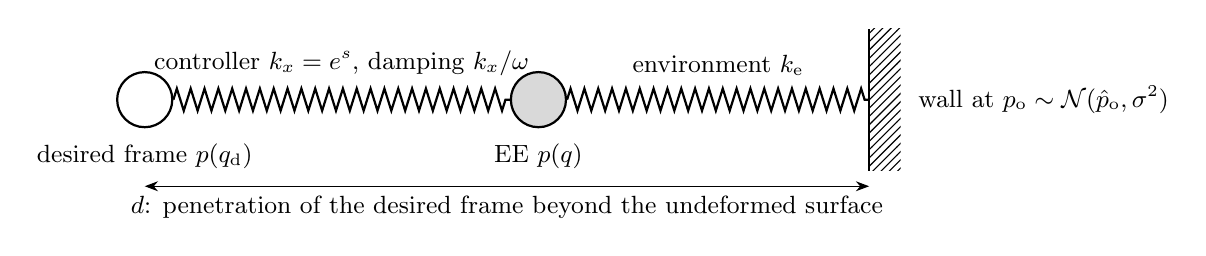
\begin{tikzpicture}[>=Stealth,font=\small,
  spring/.style={decorate,decoration={zigzag,segment length=5pt,amplitude=4pt},thick}]
  \node[circle,draw,thick,minimum size=7mm] (ref) at (0,0) {};
  \node[below=2pt of ref] {desired frame $p(\qd)$};
  \node[circle,draw,thick,fill=gray!30,minimum size=7mm] (ee) at (5,0) {};
  \node[below=2pt of ee] {EE $p(q)$};
  \draw[spring] (ref.east) -- node[above=5pt]{controller $\kx=e^{s}$, damping $\kx/\omega$} (ee.west);
  \draw[spring] (ee.east) -- node[above=5pt]{environment $\ke$} (9.2,0);
  \fill[pattern=north east lines] (9.2,-0.9) rectangle (9.6,0.9);
  \draw[thick] (9.2,-0.9) -- (9.2,0.9);
  \node[right] at (9.7,0) {wall at $p_\mathrm{o}\sim\mathcal{N}(\phat,\sigma^2)$};
  \draw[<->] (0,-1.1) -- node[below]{$d$: penetration of the desired frame beyond the undeformed surface} (9.2,-1.1);
\end{tikzpicture}
\caption{Series-spring contact model. Both springs carry the same force, so
$\kb^{-1}=\ke^{-1}+\kx^{-1}$ and $F=\kb\,d$. The resulting stiffness never exceeds the controller
stiffness.}
\label{fig:springs}
\end{figure}

\subsection{VI-MPIC model for the 2-link arm}
VI-MPIC adds the log-stiffness as a state and its rate as an input:
\begin{equation}
x=\bigl[q;\ \qd;\ F;\ s\bigr]\in\mathbb{R}^8,\qquad u=\bigl[u_q;\ u_s\bigr]=\bigl[\dqd;\ \dot s\bigr]\in\mathbb{R}^4 ,
\end{equation}
\begin{equation}\label{eq:vimpic}
\boxed{\;\dot q=u_q+\omega(\qd-q)-\omega J_0^{-1}w,\quad
\dqd=u_q,\quad
\dot F_i=\kb_i\bigl(\gamma_i\,(J_0u_q)_i+\psi\,w_i\,u_{s,i}\bigr),\quad
\dot s=u_s\;}
\end{equation}
with $\kx=e^s$, $w=F\oslash\kx$ and $\psi=1$. The stiffness-rate term follows from differentiating
$F=\kb(s)\,d$:
\begin{equation}
\dot F=\kb\,\dot d+\frac{\partial\kb}{\partial s}\dot s\,d
=\kb\,\dot d+\frac{\kb^2}{\kx}\,\frac{F}{\kb}\,\dot s
=\kb\bigl(\dot d+w\,\dot s\bigr).
\end{equation}
With the reference held, halving the stiffness halves the force, a change the frozen model
\eqref{eq:mpic} does not predict at all (Proposition~1 of \cite{notes}). Axis $x$ is the wall normal.
Axis $y$ has no environment ($\ke=0$), so $F_y$ keeps its measured value.

\subsection{Probabilistic contact gate and expected force}
Along the normal, the planned depth of the desired frame is linearised with the frozen Jacobian,
$m(\qd)=m_k+J_{0,x}(\qd-q_{\mathrm{d},k})$. The penetration is $d=m-p_\mathrm{o}$ with
$p_\mathrm{o}\sim\mathcal{N}(\phat,\sigma^2)$, and the force is $F_x=\kb\,d^+$. With $b=(m-\phat)/\sigma$:
\begin{itemize}[leftmargin=14pt]
\item \textbf{Unconditioned gate} (N27): $\gamma=\Phi(b)$, $\mathrm{E}[d^+]=\sigma\bigl(b\Phi(b)+\varphi(b)\bigr)$.
  The force state of \eqref{eq:vimpic} is then the expected force.
\item \textbf{Conditioned gate} (A3.4--A3.5). Before the first contact, ``no force measured'' means that
  the surface lies beyond the deepest contact-free point $\ell$. Conditioning on $p_\mathrm{o}\ge\ell$, with
  $a=(\ell-\phat)/\sigma$ and for $b>a$:
\begin{equation}\label{eq:cond}
\gamma=\frac{\Phi(b)-\Phi(a)}{1-\Phi(a)},\qquad
g=\mathrm{E}\bigl[d^+\,\big|\,p_\mathrm{o}\ge\ell\bigr]=\sigma\,\frac{b\bigl(\Phi(b)-\Phi(a)\bigr)+\varphi(b)-\varphi(a)}{1-\Phi(a)} .
\end{equation}
\end{itemize}
The stiffness cost also needs the \textbf{conditioned variance}, which the analysis does not give. It is
derived here and checked by Monte Carlo in Section~\ref{sec:checks}:
\begin{equation}\label{eq:var}
\begin{gathered}
\mathrm{E}\bigl[(d^+)^2\,\big|\,p_\mathrm{o}\ge\ell\bigr]=\sigma^2\,
\frac{(b^2+1)\bigl(\Phi(b)-\Phi(a)\bigr)+b\varphi(b)+(a-2b)\varphi(a)}{1-\Phi(a)},\\
\mathrm{Var}=\mathrm{E}\bigl[(d^+)^2\,\big|\,p_\mathrm{o}\ge\ell\bigr]-g^2,\qquad
\frac{\partial g}{\partial m}=\gamma,\qquad \frac{\partial \mathrm{Var}}{\partial m}=2g(1-\gamma).
\end{gathered}
\end{equation}
For $a\to-\infty$ it reduces to the rectified-Gaussian moment (N28). Before the first contact the force
state is initialised with its own expectation $\kb\,g(m_k)$ (remark in A3.2).

\subsection{Optimal control problem}
The stage cost combines the MPIC terms (N9) with the stiffness cost (N30):
\begin{align}
l&=\tfrac12\|p(q)-p_\mathrm{des}\|^2_{Q_p}+\tfrac12\|p(\qd)-p_\mathrm{des}\|^2_{Q_r}+\tfrac12\|F-\Fdes\|^2_{Q_F}\notag\\
&\quad+\tfrac12 R_q\|u_q\|^2+\tfrac12 Q_v\bigl(J_{0,x}u_q-\vapp\bigr)^2+l_s,\\
l_s&=\sum_{i}\Bigl[\tfrac12 q_F\,\kb_i^2\,\mathrm{Var}[d_i^+]+\tfrac12 q_p\,\sigma_w^2\Bigl(\frac{1-\gamma_i}{k_{x,i}^2}+\frac{\gamma_i}{(k_{x,i}+k_{\mathrm{e},i})^2}\Bigr)+\tfrac12 r_s\,u_{s,i}^2\Bigr].\label{eq:ls}
\end{align}
The first term of $l_s$ is the \emph{force risk}: the force variance grows with the stiffness and with
the contact probability. The second is the \emph{disturbance risk}: a disturbance of standard deviation
$\sigma_w$ deflects the EE by $\sigma_w/\kx$ in free space and by $\sigma_w/(\kx+\ke)$ in contact.
Different weights select the task primitives:
\begin{itemize}[leftmargin=14pt]
\item \emph{hold}: EE position;
\item \emph{guarded approach}: velocity $\vapp$ of the desired frame along the normal;
\item \emph{force primitive}: $\Fdes$ along the normal, entered once contact is measured;
\item \emph{slide}: a tangential target moving along the wall.
\end{itemize}
The constraints are $s_\mathrm{min}\le s\le s_\mathrm{max}$, the stiffening bound
$\dot s\le 0.95\cdot\tfrac85\,\omega$ (Proposition~A.3.4), and $\dot s\ge -40$\,1/s for softening. The
floor follows from requiring an overdamped loop, $k\ge4\omega^2m_\mathrm{eff}$ (N15).

\subsection{Implementation in GRAMPC}
The problem is a problem description for GRAMPC 2.3 \cite{grampc} (\texttt{probfct\_VI\_MPIC.c}) with analytic adjoint
products (N20, N21), including the gate derivatives $\partial\gamma/\partial m=\varphi(b)/\bigl(\sigma(1-\Phi(a))\bigr)$
and the derivatives of \eqref{eq:ls}. Before each step (\emph{prestep}) $J_0$, $J_0^{-1}$, the depth
$m_k$, the belief $(\phat,\sigma,\ell)$ and the primitive weights are written into the user parameters.
After each step (\emph{poststep}) $\qd$ and $s$ are remembered, so the reference the low-level loop
receives is exactly the planned one. The belief is updated as in Table~A.5:
\begin{itemize}[leftmargin=14pt]
\item before contact: the prior, with $\ell$ the deepest depth reached;
\item in contact: $\phat=p_x-F_x/\ke$ with $\sigma=\SI{1}{mm}$;
\item after a loss of contact: $\sigma$ inflated to \SI{5}{mm}.
\end{itemize}
The same file runs classical MPIC: with fixed stiffness and the measured gate, \eqref{eq:vimpic} reduces
to \eqref{eq:mpic}. Two numerical details were necessary:
\begin{itemize}[leftmargin=14pt]
\item the stiffness rate is input-scaled by 20 for the gradient method;
\item for fixed gains it is removed from the model, because a pinned input with a non-zero gradient spoils
  GRAMPC's explicit line search.
\end{itemize}
Fig.~\ref{fig:structure} shows the closed loop.

\begin{figure}[!htbp]
\centering
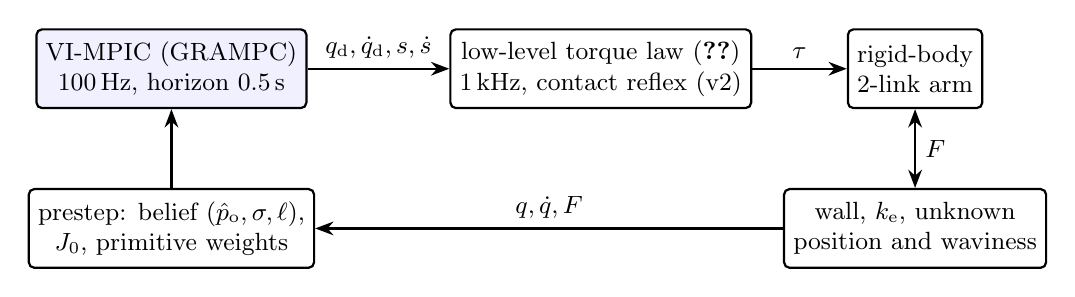
\begin{tikzpicture}[>=Stealth,font=\small,node distance=6mm and 10mm,
  blk/.style={draw,thick,rounded corners=2pt,align=center,minimum height=10mm,fill=white},
  hl/.style={blk,fill=blue!6}]
  \node[hl] (mpc) {VI-MPIC (GRAMPC)\\ 100\,Hz, horizon 0.5\,s};
  \node[blk,right=18mm of mpc] (ll) {low-level torque law \eqref{eq:torque}\\ 1\,kHz, contact reflex (v2)};
  \node[blk,right=12mm of ll] (arm) {rigid-body\\ 2-link arm};
  \node[blk,below=10mm of arm] (wall) {wall, $\ke$, unknown\\ position and waviness};
  \node[blk,below=10mm of mpc] (bel) {prestep: belief $(\phat,\sigma,\ell)$,\\ $J_0$, primitive weights};
  \draw[->,thick] (mpc) -- node[above]{$\qd,\dqd,s,\dot s$} (ll);
  \draw[->,thick] (ll) -- node[above]{$\tau$} (arm);
  \draw[<->,thick] (arm) -- node[right]{$F$} (wall);
  \draw[->,thick] (wall.west) -- node[above]{$q,\dot q,F$} (bel.east);
  \draw[->,thick] (bel) -- (mpc);
\end{tikzpicture}
\caption{Closed loop of the study. Only the MPC block differs between classical MPIC and VI-MPIC; the
contact reflex is an option of the low-level loop for every controller.}
\label{fig:structure}
\end{figure}

%==============================================================================
\section{Evaluation methodology}\label{sec:eval}

\subsection{Plant}
The plant is \emph{not} the MPC model. It is the rigid-body 2-link arm, with links of \SI{0.2}{m} and
\SI{0.5}{kg} in the horizontal plane, driven by the torque law \eqref{eq:torque}. It keeps the inertia the
MPC neglects; its effective mass along the wall normal is 0.23--0.32\,kg. It is integrated semi-implicitly
(damping implicit) at \SI{0.2}{ms}. The wall is a spring-damper ($\ke=\SI{5000}{N/m}$,
$c_\mathrm{e}=\SI{10}{Ns/m}$) at $\phat+\Delta$, with the offset $\Delta$ unknown to the controller. The
force is measured perfectly at the MPC rate. Appendix~\ref{app:params} lists all parameters.

\subsection{Tasks}
\begin{description}[leftmargin=10pt,font=\normalfont\bfseries]
\item[Impact task.] The arm runs through three phases:
  \begin{enumerate}[leftmargin=14pt]
  \item 0--1\,s: hold $(0.22,0)$\,m while a \SI{5}{N} push along the wall normal acts during 0.2--0.7\,s;
  \item guarded approach: the desired frame moves towards the wall at $\vapp\in\{0.1,0.2,0.3\}$\,m/s;
  \item once contact is measured ($F>\SI{0.5}{N}$): press with $\Fdes=\SI{5}{N}$.
  \end{enumerate}
\item[Sliding task] (E3 of the notes). After the impact task's contact, wait \SI{0.4}{s}, then slide
  \SI{5}{cm} along the wall at \SI{5}{cm/s} while keeping \SI{5}{N}. The wall has a sinusoidal waviness of
  \SI{2}{mm} amplitude and \SI{5}{cm} wavelength that the controller does not know.
\end{description}

\subsection{Uncertainty and metrics}
The belief is $\phat=\SI{0.30}{m}$, $\sigma=\SI{10}{mm}$. The true wall lies at
$\Delta\in\{-20,-15,\dots,20\}$\,mm (9 offsets; 5 for sliding). Every controller runs with 10 gradient
iterations per step, the real-time setting of the notes, and again with 50. The metrics are:
\begin{itemize}[leftmargin=14pt]
\item \emph{free-motion tracking error}: RMS EE position error over 0.2--1.0\,s;
\item \emph{worst force peak}: the largest contact force, worst case over the offsets;
\item \emph{unsettled runs}: force RMS error above \SI{1}{N} over the last \SI{0.5}{s}, or no contact;
\item for sliding, the \emph{normal-force RMS error} while sliding and the tangential RMS error.
\end{itemize}

\subsection{Controllers}
\begin{table}[!htbp]
\centering\small
\caption{Controllers. Every controller also runs with the \SI{1}{kHz} contact reflex (suffix \texttt{\_rfx}).}
\label{tab:controllers}
\begin{tabularx}{\linewidth}{@{}>{\raggedright\arraybackslash}p{3.4cm}>{\raggedright\arraybackslash}X>{\raggedright\arraybackslash}p{1.9cm}>{\raggedright\arraybackslash}X@{}}
\toprule
name & stiffness & gate & purpose \\
\midrule
\texttt{mpic\_k*} & fixed, 300 \dots 10000\,N/m & measured & classical MPIC, Pareto sweep \\
\texttt{vimpic} & optimised & conditioned & VI-MPIC as proposed (first draft) \\
\texttt{vimpic\_nopsi}, \texttt{\_measgate}, \texttt{\_uncond} & optimised & varies & ablations: no $w\odot\dot s$, measured or unconditioned gate \\
\texttt{vimpic\_cg} \dots\ \texttt{vimpic\_v2} & optimised & see Sec.~\ref{sec:v2} & improvement ladder \\
\texttt{sched\_dist} & $10^4\to300$\,N/m between $3\sigma$ and $1\sigma$ before $\phat$ & measured & simple anticipatory schedule \\
\texttt{sched\_contact} & $10^4$\,N/m until contact, hold 0.2\,s, then to 900\,N/m at 3\,1/s & measured & hand-made counterpart of v2 \\
\bottomrule
\end{tabularx}
\end{table}

\subsection{Model checks}\label{sec:checks}
\begin{itemize}[leftmargin=14pt]
\item \emph{Adjoints}: GRAMPC's finite-difference gradient check passes in every gate mode. The single
  remaining entry is at the finite-difference noise floor.
\item \emph{Gate moments}: \eqref{eq:cond} and \eqref{eq:var} are checked against $4\cdot10^6$ Monte Carlo
  samples.
\item \emph{E1, force model}: on the rigid-body plant the reference is held in contact while the
  stiffness ramps from 5000 to 1000\,N/m.
\item \emph{E5, convergence}: selected states are re-solved with 200 extra iterations.
\end{itemize}

%==============================================================================
\section{Results of the proposed VI-MPIC (first draft)}\label{sec:v1}

\subsection{Model checks}
The conditioned moments agree with Monte Carlo, for example $\sqrt{\mathrm{Var}}=2.886$\,mm against
2.887\,mm, and $\gamma=\partial g/\partial m$ to five digits. Fig.~\ref{fig:e1} confirms the stiffness-rate
term. With the reference held, the force falls from 5.00 to 1.66\,N. The model with $w\odot\dot s$
predicts the final value to 0.003\,N, while the frozen model of classical MPIC is off by 3.34\,N. During
the ramp, however, the plant lags the prediction by up to 0.63\,N ($\dot s=-8$\,1/s) and 1.63\,N
($\dot s=-40$\,1/s), i.e.\ by 20--30\,ms. Claim~C1 holds quasi-statically.

The effective mass along the normal is 0.23--0.32\,kg, so the free-space floor (N15) is \SI{127}{N/m}.
\emph{In contact} the wall adds stiffness, and an overdamped contact mode,
$m\ddot x+(k/\omega)\dot x+(k+\ke)x=0$ with $\zeta\ge1$, requires
\begin{equation}\label{eq:floor}
k\ \ge\ 2\omega^2m\Bigl(1+\sqrt{1+\ke/(\omega^2m)}\Bigr)=\SI{864}{N/m}.
\end{equation}

\begin{figure}[!htbp]
\centering
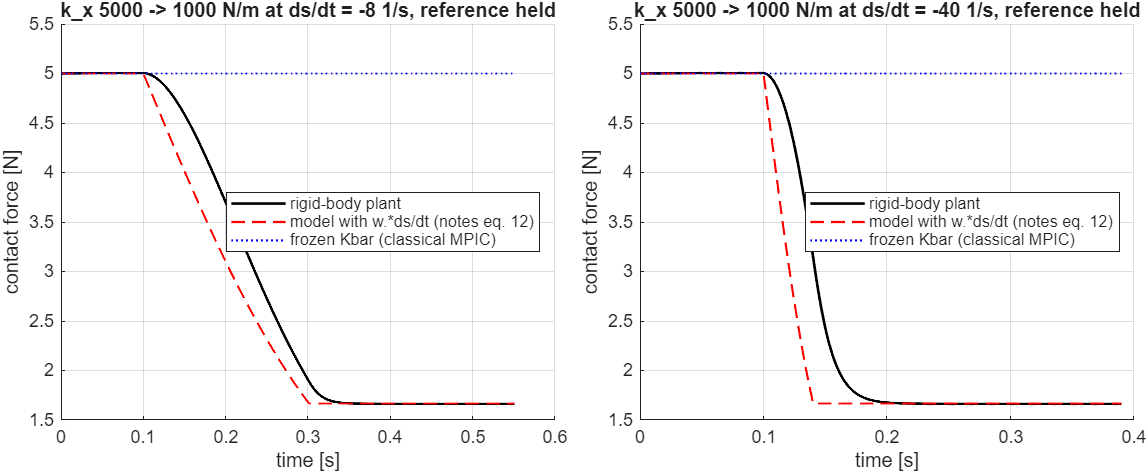
\includegraphics[width=0.95\linewidth]{vi_e1_force_model.png}
\caption{E1: contact force on the rigid-body plant while the normal stiffness ramps from 5000 to
1000\,N/m with the reference held. The model with the stiffness-rate term gets the final force right; the
frozen-$\Kbar$ model of classical MPIC predicts no change.}
\label{fig:e1}
\end{figure}

\subsection{Benchmark}
Fig.~\ref{fig:v1pareto} and Table~\ref{tab:v1} show the result of 864 runs. VI-MPIC tracks like the stiffest
fixed gain in free motion, by construction, since it sits at $k_\mathrm{max}$ away from the wall. Its worst
force peak, however, is higher than that of every fixed gain at every speed in the real-time setting: it
lies \emph{above} the front. With 50 iterations every controller pushes harder into the contact, and
VI-MPIC beats the stiff gains only at 0.3\,m/s. No ablation is better in every setting. Removing
$w\odot\dot s$ looks best with 10 iterations, but with 50 iterations the force is unsettled in 23 of 27
runs.

\begin{table}[!htbp]
\centering\small
\caption{First draft, worst force peak in N at 0.1\,/\,0.2\,/\,0.3\,m/s ($\Fdes=\SI{5}{N}$); tracking RMS at
0.2\,m/s; number of unsettled runs (of 27) in brackets.}
\label{tab:v1}
\begin{tabular}{@{}lcccc@{}}
\toprule
controller & tracking [mm] & 10 iterations & 50 iterations & solve [ms], 10 it \\
\midrule
MPIC 300\,N/m & 5.69 & 5.0 / 7.4 / 11.4 & 6.8 / 7.7 / 11.2 & 0.27--0.37 \\
MPIC 800\,N/m & 2.15 & 5.0 / 7.1 / 12.0 & 9.1 / 9.3 / 12.2 (1) & 0.26--0.37 \\
MPIC 3000\,N/m & 0.61 & 5.1 / 8.8 / 13.8 & 11.6 / 11.6 / 16.4 (5) & 0.26--0.37 \\
MPIC 10000\,N/m & 0.32 & 5.2 / 9.4 / 14.1 & 5.9 / 9.8 / 19.2 & 0.26--0.38 \\
\midrule
\textbf{VI-MPIC} & 0.33 & \textbf{7.4 / 14.1 / 19.5} & 9.2 / 10.7 / 14.9 (1) & 0.47--0.70 \\
\quad without $w\odot\dot s$ & 0.32 & 5.0 / 7.8 / 18.4 & 25.5 / 14.6 / 21.5 (23) & 0.47--0.75 \\
\quad measured gate & 0.32 & 7.0 / 16.6 / 27.8 & 12.5 / 11.4 / 17.9 & 0.26--0.37 \\
\quad unconditioned gate & 0.33 & 7.2 / 14.0 / 19.3 & 7.1 / 10.4 / 13.4 & 0.47--0.68 \\
schedule on distance & 0.32 & 5.0 / 8.9 / 12.9 & 11.9 / 12.1 / 12.4 (1) & 0.26--0.51 \\
\bottomrule
\end{tabular}
\end{table}

\begin{figure}[!htbp]
\centering
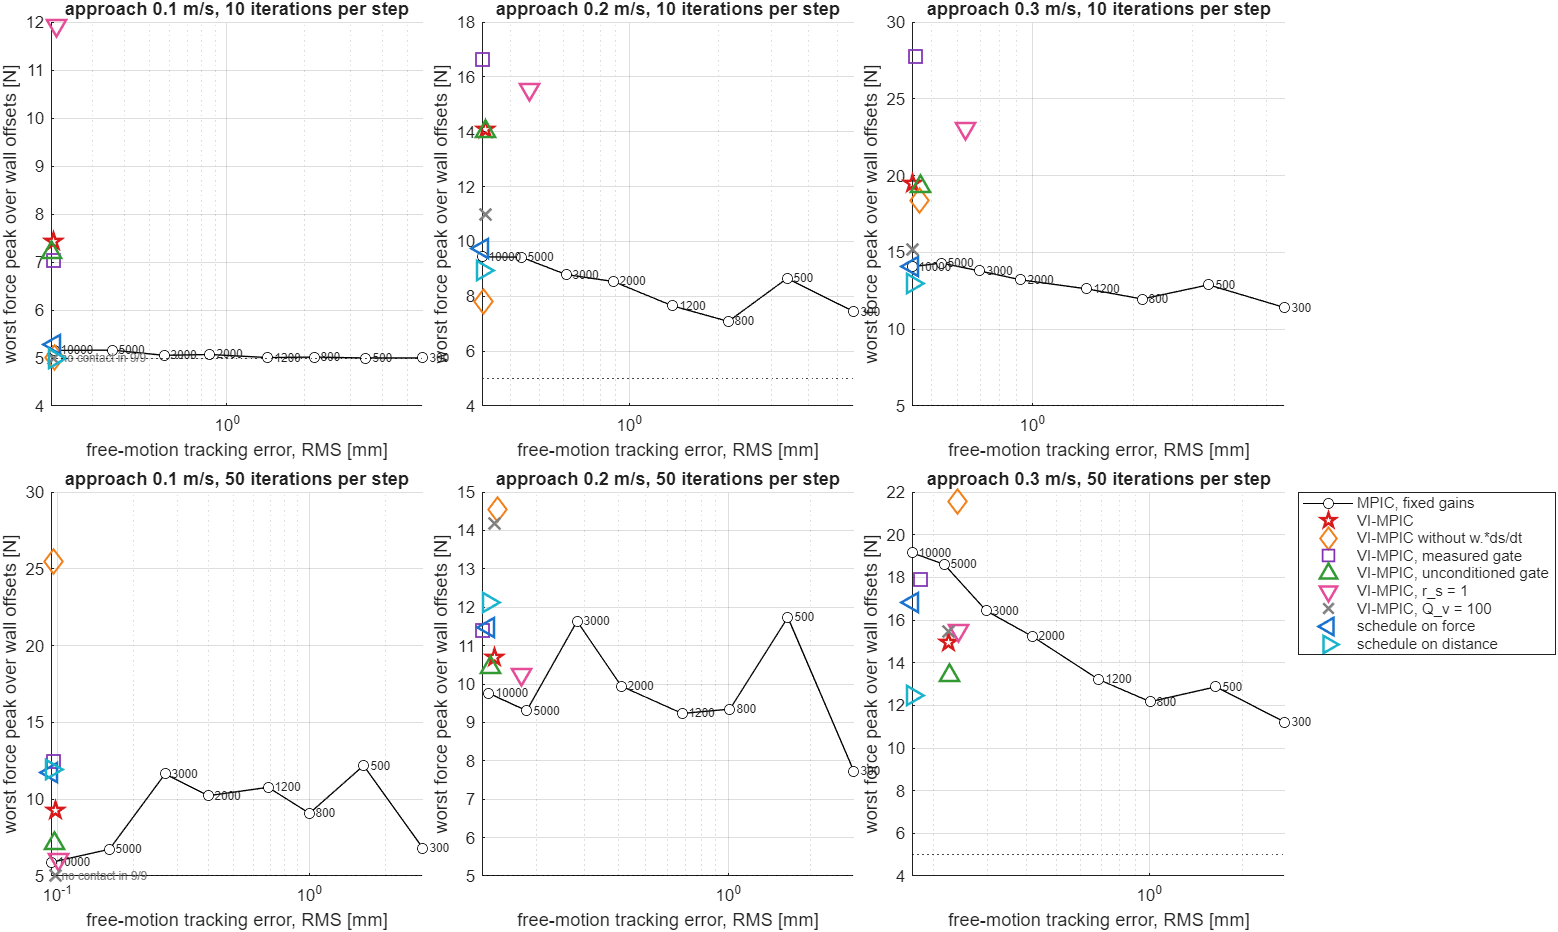
\includegraphics[width=\linewidth]{vi_pareto.png}
\caption{First draft: worst force peak over the wall offsets against free-motion tracking error. Black:
fixed-gain MPIC, labelled with the stiffness in N/m. Top row: 10 iterations per step; bottom: 50.}
\label{fig:v1pareto}
\end{figure}

\subsection{Issues found while drafting}\label{sec:issues}
Building a working first draft already required changes to the task specification and exposed several
properties of the formulation:
\begin{enumerate}[label=I\arabic*.]
\item \emph{An expected-force state must not drive an EE position cost.} Before contact the model pushes
  $q$ back by the expected deflection $J_0^{-1}F/\kx$, which is about \SI{10}{mm} at 300\,N/m. A cost on
  $p(q)$ moves the reference ahead, and the real arm, which has no contact yet, follows it into the wall.
  The approach is therefore specified on the desired frame.
\item \emph{The approach must be a speed, not a time-indexed target.} A delayed reference otherwise
  sprints after its target. With the force cost active before contact, the expected-force model pulls the
  reference towards the believed wall.
\item \emph{The risk cost acts on the motion and can stall it.} $\mathrm{Var}[d^+]$ depends on the planned
  depth, so stopping is cheaper than softening. With a weak approach drive VI-MPIC never touches the wall
  at 0.1\,m/s.
\item \emph{The conditioned gate can report contact that is not there.} After a bounce, $\kb\,g(m_k)$
  reads ``pressing'' while the arm is away.
\item \emph{Numerics.} The stiffness rate needs input scaling. A pinned input with a non-zero gradient
  stalls GRAMPC's explicit line search. The real-time iterate is far from converged at the impact: E5
  shows that 55--99\,\% of the cost there would be removed by 200 more iterations.
\end{enumerate}

\textbf{Answer to Q1.} VI-MPIC as proposed does not give an advantage over classical MPIC on this robot. It
lies above the fixed-gain front at impact, and its ablations do not rank consistently.

%==============================================================================
\section{Diagnosis: why the first draft hit harder}\label{sec:diag}

The fine plant logs (0.2\,ms) around the first contact show what the controllers do with the reference
right after the impact (Table~\ref{tab:diag}).

\begin{table}[!htbp]
\centering\small
\caption{Reference velocity along the normal at the first MPC steps after the impact (0.2\,m/s, 10
iterations, 9 offsets).}
\label{tab:diag}
\begin{tabularx}{\linewidth}{@{}>{\raggedright\arraybackslash}p{3.6cm}>{\raggedright\arraybackslash}Xll@{}}
\toprule
controller & reference velocity after contact & force peak & time of peak \\
\midrule
MPIC 300 and 10000\,N/m & $-0.044$ to $+0.006$\,m/s at the next step & 4.8--9.4\,N & 7--9\,ms \\
VI-MPIC, first draft & $+0.11$ to $+0.20$\,m/s, then up to $+0.18$\,m/s & 9.2--14.1\,N & 11--26\,ms \\
VI-MPIC v2 + reflex & stopped at touch by the reflex & 4.9\,N (no overshoot) & -- \\
\bottomrule
\end{tabularx}
\end{table}

\textbf{Fixed gains} stop the reference at the next MPC sample. For a stiff gain the force peak then
depends mainly on how long the reference runs on into the wall before that sample: 9.4\,N after 7.6\,ms,
5.1\,N after 2.6\,ms. This \emph{detection delay} of up to one sampling period explains why the worst
case over the offsets depends on the sampling phase. For a soft gain, the inertial spike of the arm adds
to it.

\textbf{VI-MPIC keeps pushing} at full approach speed for one or two more steps, for two reasons:
\begin{enumerate}[label=(\alph*)]
\item \emph{The probabilistic gate in contact under-predicts the force rate.} Right after touch the
  reference is only about \SI{1}{mm} past the estimated surface, which has $\sigma=\SI{1}{mm}$, so
  $\gamma\approx0.6$--$0.9$. The model expects the force to build more slowly than it does.
\item \emph{Push and soften.} The stiffness cost keeps softening in contact. Through $w\odot\dot s$ the
  model expects the softening to cancel the push. In the plant the push acts at once, while the softening
  takes effect only after the arm has moved back against its inertia (E1). Meanwhile the co-scheduled
  damping $K_\mathrm{D}=K_\mathrm{P}/\omega$ drops with the stiffness.
\end{enumerate}

%==============================================================================
\section{Improvements: what and why}\label{sec:v2}

Each change addresses a mechanism of Section~\ref{sec:diag} or Section~\ref{sec:issues}, and each is a
switchable option, so its effect can be measured alone.

\paragraph{1. Measured gate once in contact.}
\emph{What:} $\gamma=1$ in the force row as soon as contact is measured; the probabilistic gate is used only
before contact. \emph{Why:} once a force is measured the surface position is known, and keeping a gate
with $\sigma_\mathrm{meas}$ only adds a model error at the moment that matters most, reason~(a).

\paragraph{2. No stiffness actuation during the impact transient.}
\emph{What:} in the contact primitive, $\dot s=0$ for $T_\mathrm{h}=\SI{0.2}{s}$ after the first contact;
afterwards $|\dot s|\le r_\mathrm{c}=3$\,1/s. \emph{Why:} reason~(b). The stiffness-rate term is exact only
quasi-statically. During the first tens of milliseconds the optimiser would use the stiffness as a fast
force actuator that the arm cannot follow.

\paragraph{3. Contact-aware stiffness floor.}
\emph{What:} $k_\mathrm{min}=\SI{900}{N/m}$ instead of 300\,N/m. \emph{Why:} by \eqref{eq:floor} a lower
stiffness makes the contact mode underdamped. Held at such a stiffness, the arm bounces, and a converged
MPC over-drives it.

\paragraph{4. Force risk only in contact.}
\emph{What:} $q_F=0$ before contact. In contact, $\sigma$ in the risk term is the unknown surface variation
along the path ($\sigma_\mathrm{c}=\SI{2}{mm}$) instead of the position belief. \emph{Why:} with the
reflex below, a stiff arm meets the wall best, because its damping stops it fastest. Softening before
contact then only hurts. The useful stiffness modulation is in sustained contact over an uncertain surface.

\paragraph{5. Force-state reset after a loss of contact.}
\emph{What:} $F(t_k)=0$ instead of $\kb\,g(m_k)$ once contact has been lost. \emph{Why:} the
initialisation of A3.2 removes the mismatch only for the quasi-static tip lag. After a bounce it reports
pressing while the arm is away (issue I4).

\paragraph{6. Contact reflex in the low-level loop (all controllers).}
\emph{What:} if the force crosses the contact threshold inside an MPC interval that was planned without
contact, the \SI{1}{kHz} loop stops the reference and the stiffness at that instant instead of driving on
until the next MPC sample. \emph{Why:} the detection delay sets the impact peak (Section~\ref{sec:diag}).
This is a change of the low-level loop, not of the MPC, so it is applied to every baseline as well.

\medskip
\textbf{VI-MPIC v2} has changes 1--5; \textbf{v2 + reflex} adds change 6. To test whether the
\emph{optimisation} matters, v2 is compared with \texttt{sched\_contact}, a hand-made schedule that
follows the same stiffness logic.

%==============================================================================
\section{Results of the improved VI-MPIC}\label{sec:v2res}

\subsection{Improvement ladder}
Fig.~\ref{fig:ladder} and Table~\ref{tab:ladder} add the changes one at a time. At 0.2\,m/s with 10 iterations:
\begin{itemize}[leftmargin=14pt]
\item the measured gate alone changes little (14.1\,N);
\item holding the stiffness in contact is the key VI-specific fix (14.1\,$\to$\,7.8\,N);
\item with 50 iterations the hold needs the floor (18.2\,$\to$\,9.9\,N).
\end{itemize}
The reflex lowers every controller: the fixed 10\,kN/m gain goes from 9.4 to 5.2\,N, v2 from 10.0 to
5.5\,N. With the reflex, staying stiff until contact (change~4) makes v2 the most robust VI variant at 50
iterations: 7.7\,N against 8.2--12.5\,N for the variants that soften before contact.

\begin{figure}[!htbp]
\centering
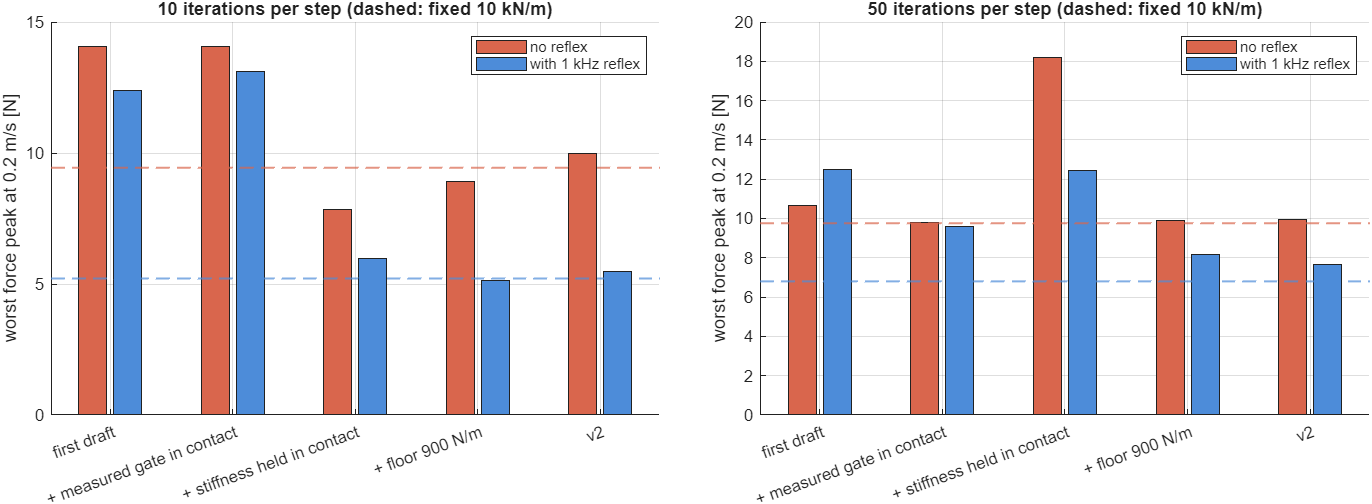
\includegraphics[width=\linewidth]{vi2_ladder.png}
\caption{Improvement ladder at 0.2\,m/s: worst force peak after each change, without and with the
reflex. Dashed: the fixed 10\,kN/m gain without and with the reflex.}
\label{fig:ladder}
\end{figure}

\begin{table}[!htbp]
\centering\small
\caption{Impact task, worst force peak in N at 0.1\,/\,0.2\,/\,0.3\,m/s; unsettled runs (of 27) in
brackets. All VI variants and schedules track like the stiffest gain (0.32--0.33\,mm at 10 iterations,
0.13--0.15\,mm at 50).}
\label{tab:ladder}
\setlength{\tabcolsep}{4pt}
\begin{tabular}{@{}lcccc@{}}
\toprule
controller & 10 it & 10 it + reflex & 50 it & 50 it + reflex \\
\midrule
VI-MPIC, first draft & 7.4/14.1/19.5 & 6.6/12.4/17.6 & 9.2/10.7/14.9 (1) & 9.2/12.5/11.9 \\
+ measured gate in contact & 7.5/14.1/19.5 & 6.5/13.1/17.6 & 7.6/9.8/14.4 & 9.1/9.6/12.8 \\
+ stiffness held in contact & 5.0/7.8/13.6 & 5.0/6.0/8.0 & 12.4/18.2/17.8 (4) & 9.7/12.5/12.6 (1) \\
+ floor 900\,N/m & 5.1/8.9/13.3 & 5.1/5.1/5.0 & 7.4/9.9/14.6 & 11.2/8.2/9.1 \\
\rowcolor{blue!6}\textbf{v2} & 5.3/10.0/16.3 & \textbf{5.2/5.5/5.4} & 6.0/10.0/17.0 & \textbf{7.0/7.7/6.4} \\
\midrule
schedule on distance & 5.0/8.9/12.9 & 5.1/6.2/8.4 & 11.9/12.1/12.4 (1) & 12.9/13.5/12.6 \\
schedule after contact & 5.0/9.4/14.1 & 5.0/5.0/5.1 & 8.2/10.9/19.2 (1) & 11.7/12.1/9.8 (3) \\
MPIC 300\,N/m & 5.0/7.4/11.4 & 5.0/5.0/7.1 & 6.8/7.7/11.2 & 8.2/10.4/8.8 \\
MPIC 800\,N/m & 5.0/7.1/12.0 & 5.0/5.0/5.9 & 9.1/9.3/12.2 (1) & 11.9/13.0/12.7 (2) \\
MPIC 3000\,N/m & 5.1/8.8/13.8 & 5.1/5.1/5.1 & 11.6/11.6/16.4 (5) & 10.9/10.8/10.5 (7) \\
MPIC 10000\,N/m & 5.2/9.4/14.1 & 5.2/5.2/5.2 & 5.9/9.8/19.2 & 6.9/6.8/6.7 \\
\bottomrule
\end{tabular}
\end{table}

\subsection{Impact: the fixed-gain front with and without the reflex}
Fig.~\ref{fig:impact} shows the main effect of the reflex. With 10 iterations it moves the entire
fixed-gain front down to about 5\,N, so the impact trade-off that VI-MPIC was meant to remove disappears.
With 50 iterations all controllers are noisier. v2 with the reflex is then the best controller at
0.3\,m/s (6.4\,N) and close to the stiff fixed gain at 0.1 and 0.2\,m/s (7.0 and 7.7\,N against 6.9 and
6.8\,N).

\begin{figure}[!htbp]
\centering
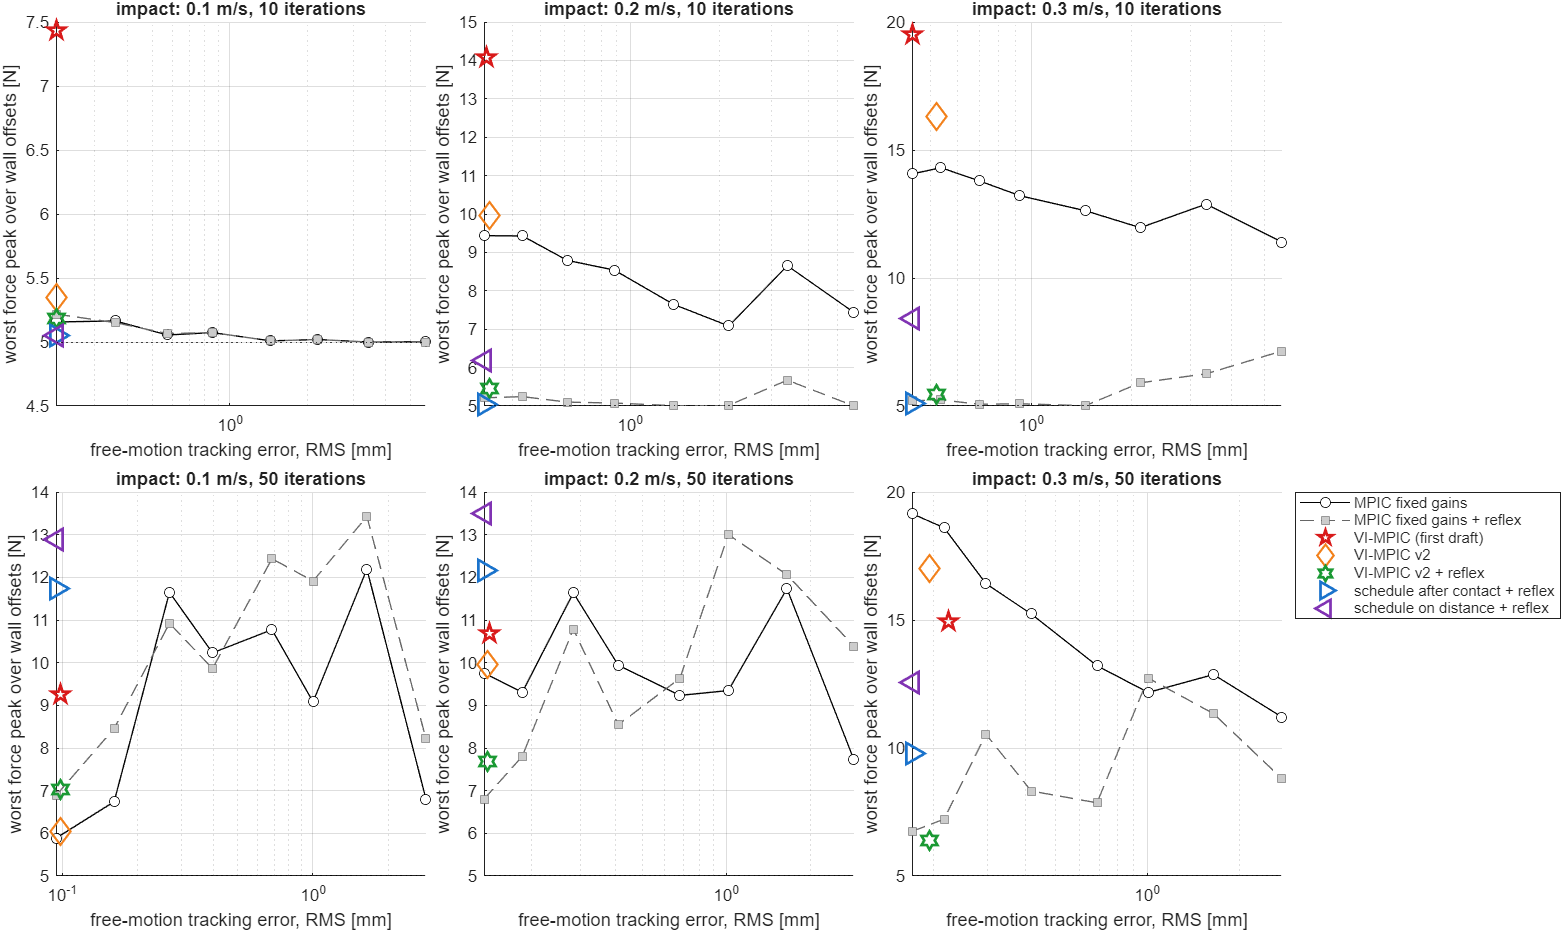
\includegraphics[width=\linewidth]{vi2_impact_pareto.png}
\caption{Impact task: worst force peak against free-motion tracking error. Black: fixed gains without the
reflex; grey dashed: with the reflex. Top: 10 iterations; bottom: 50.}
\label{fig:impact}
\end{figure}

\subsection{Sliding over an unknown waviness}
In sustained contact the stiffness genuinely matters (Fig.~\ref{fig:slide}, Table~\ref{tab:slide}). For fixed
gains the normal-force error while sliding grows with the stiffness, from 0.12\,N at 300\,N/m to 0.68\,N
at 10\,kN/m, while the tracking error falls from 5.69 to 0.32\,mm. v2 with the reflex tracks like the
stiffest gain and halves its sliding force error. A fixed gain needs about 2000\,N/m to match 0.34\,N, and
then tracks 2.7 times worse. v2 therefore lies clearly below the fixed-gain front, together with the
hand-made schedule. The first draft is worse: its impacts reach 12\,N and its force errors 0.41\,N.

\begin{table}[!htbp]
\centering\small
\caption{Sliding task, 10 iterations, 5 wall offsets. Sliding force RMS error: mean (worst) over the
offsets.}
\label{tab:slide}
\setlength{\tabcolsep}{4pt}
\begin{tabular}{@{}lccccc@{}}
\toprule
controller & tracking & impact peak & sliding force & worst & $k$ while \\
 & [mm] & [N] & RMS [N] & deviation [N] & sliding [N/m] \\
\midrule
MPIC 10000\,N/m + reflex & 0.32 & 6.18 & 0.68 (0.70) & 1.18 & 10000 \\
MPIC 3000\,N/m + reflex & 0.61 & 5.75 & 0.42 (0.45) & 0.75 & 3000 \\
MPIC 2000\,N/m + reflex & 0.88 & 5.61 & 0.35 (0.38) & 0.61 & 2000 \\
MPIC 1200\,N/m + reflex & 1.40 & 5.46 & 0.28 (0.30) & 0.49 & 1200 \\
MPIC 300\,N/m + reflex & 5.69 & 5.40 & 0.12 (0.12) & 0.20 & 300 \\
VI-MPIC first draft + reflex & 0.33 & 12.06 & 0.41 (0.59) & 2.23 & 1899 \\
\rowcolor{blue!6}\textbf{VI-MPIC v2 + reflex} & 0.33 & 6.07 & \textbf{0.34 (0.36)} & 0.74 & 1598 \\
schedule after contact + reflex & 0.32 & 5.64 & 0.30 (0.31) & 0.93 & 1561 \\
VI-MPIC v2, no reflex & 0.33 & 9.98 & 0.35 (0.37) & 0.72 & 1595 \\
\bottomrule
\end{tabular}
\end{table}

\begin{figure}[!htbp]
\centering
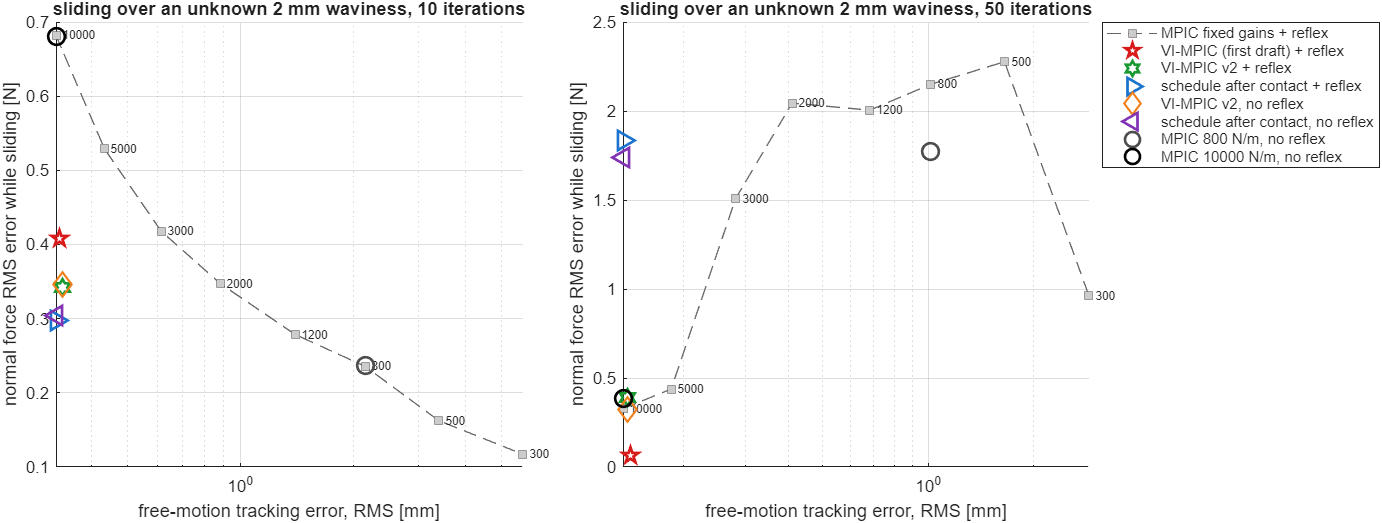
\includegraphics[width=\linewidth]{vi2_slide_pareto.png}
\caption{Sliding task: normal-force RMS error while sliding against free-motion tracking error. Grey
dashed: fixed gains with the reflex. Left: 10 iterations; right: 50 (see
Section~\ref{sec:limitcycle}).}
\label{fig:slide}
\end{figure}

\begin{figure}[!htbp]
\centering
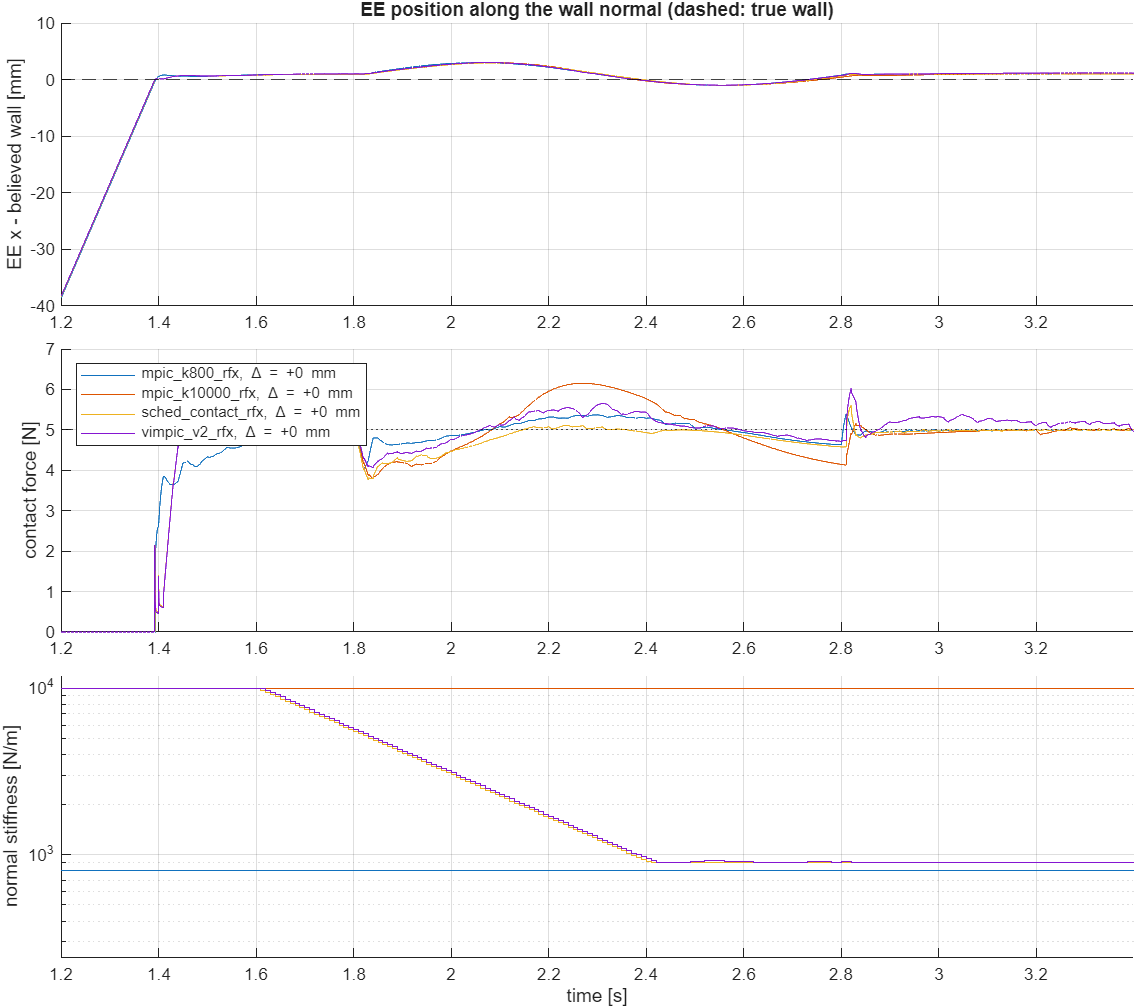
\includegraphics[width=0.74\linewidth]{vi2_slide_runs.png}
\caption{Sliding task, wall at $\phat$, 10 iterations. v2 and the schedule follow almost the same
stiffness trajectory: stiff until contact, held for 0.2\,s, then softened at the rate limit to the
floor. The stiff fixed gain swings between 4.1 and 6.1\,N over the waviness.}
\label{fig:sliderun}
\end{figure}

\subsection{Computation}
With 10 iterations the median solve time of v2 is 0.46\,ms per step. The first draft needs 0.66\,ms and
classical MPIC about 0.4\,ms. The stiffness is a decision variable only before contact and during the
slow adaptation. With 50 iterations the medians are 1.3--2.1\,ms (MPIC) and 1.9--3.5\,ms (VI-MPIC).

%==============================================================================
\section{Discussion}\label{sec:disc}

\subsection{What the stiffness optimisation adds}
In the sliding task, v2 and the hand-made schedule end up with the same stiffness trajectory. The
schedule's force error is even slightly lower (0.30 vs 0.34\,N). This is structural. For steady contact
($\gamma=1$, $\mathrm{Var}=\sigma^2$), Proposition~3 of the notes gives the minimiser of the stiffness cost:
\begin{equation}\label{eq:kstar}
k_x^\star=\frac{q_p\,\sigma_w^2}{q_F\,\sigma^2\,\ke^3}.
\end{equation}
With the weights of this study ($q_p=2\cdot10^4$, $\sigma_w=\SI{5}{N}$, $q_F=0.5$, $\sigma=\SI{2}{mm}$) the
optimum depends on the environment as follows:

\begin{center}\small
\begin{tabular}{@{}lccccc@{}}
\toprule
$\ke$ [N/m] & 5000 & 2000 & 1000 & 500 & 300 \\
$k_x^\star$ [N/m] & 2 & 31 & 250 & 2000 & 9259 \\
\bottomrule
\end{tabular}
\end{center}

On a wall much stiffer than the controller the optimum lies far below any admissible stiffness. VI-MPIC
therefore always plans ``soften to the floor as fast as allowed'', which a switch reproduces. The
optimisation does more than a switch only for soft environments, here $\ke<\SI{652}{N/m}$ (sponges,
tissue, a human), or with large disturbances in contact. Its remaining advantages are:
\begin{itemize}[leftmargin=14pt]
\item the stiffness follows from the uncertainty model instead of a hand-tuned switch;
\item anticipation before contact, which pays without a reflex: the anticipatory variant with the floor
  matches or beats the stiff fixed gain at 0.2 and 0.3\,m/s.
\end{itemize}

\subsection{Converged MPIC limit-cycles in sustained contact}\label{sec:limitcycle}
With 50 iterations, every controller whose contact stiffness is at most 3000\,N/m stops settling in the
sliding task. This affects classical fixed gains and v2 alike; only the 10\,kN/m gain stays clean. The
force oscillates with a period of two to three samples. For 3000\,N/m it swings between 0 and 15\,N, with
33 losses of contact per second (Fig.~\ref{fig:lc}).

Changing the weight on $\dqd$ from 0.01 to 1 does not remove the oscillation. The cause is the model: the
force row $\dot F=\kb J_0\dqd$ assumes the force follows the reference instantly, while the contact mode
of the arm lags by $\tau_\mathrm{c}=(k/\omega)/(k+\ke)\approx15$--$70$\,ms. A converged solver corrects
almost dead-beat on a model without that lag. Ten iterations under-converge and so act as a low-gain
filter, and the first draft's gate $\gamma<1$ in contact acts the same way. Both are accidents, not a
design.

\begin{figure}[!htbp]
\centering
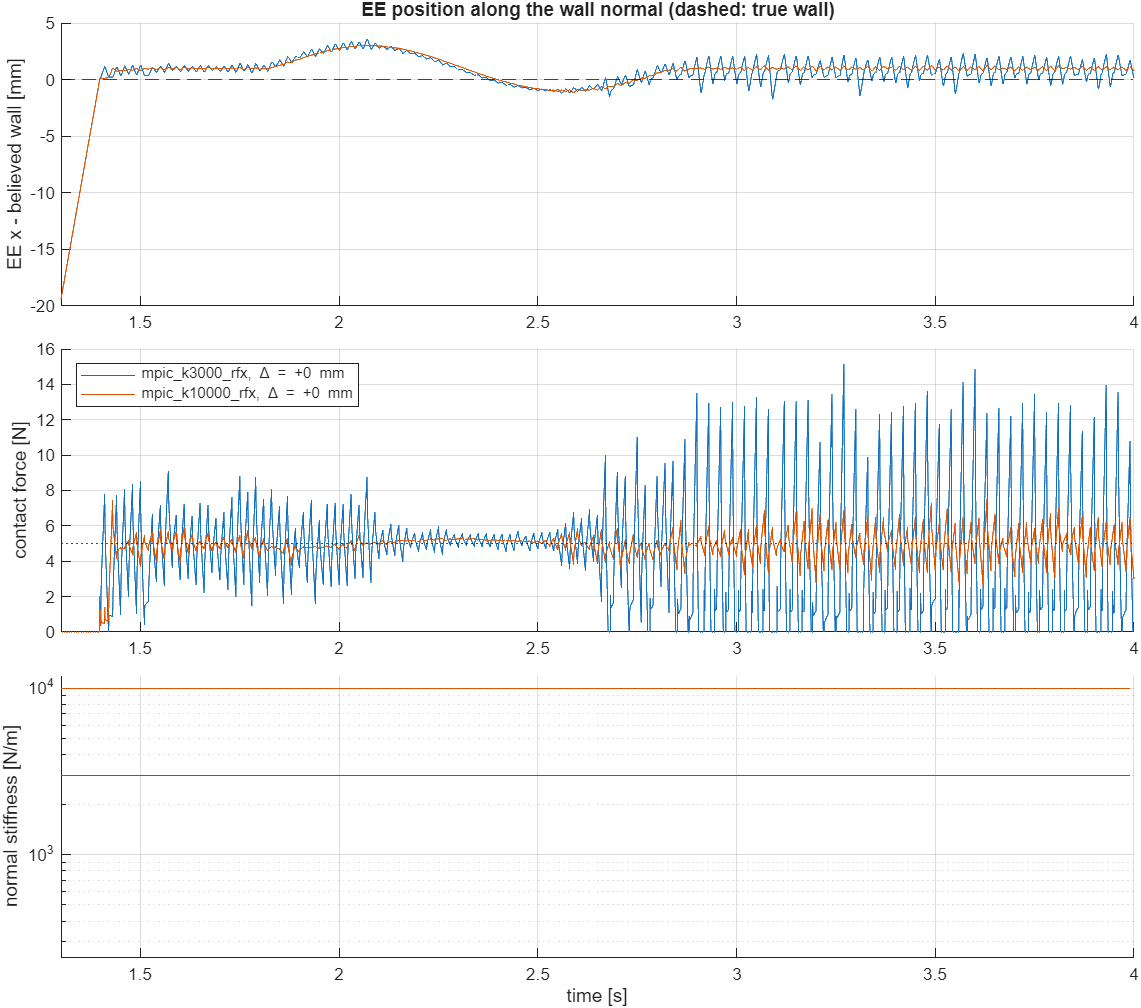
\includegraphics[width=0.74\linewidth]{vi2_limit_cycle.png}
\caption{Sliding task with 50 iterations: the fixed 3000\,N/m gain limit-cycles (0--15\,N, repeated
loss of contact); the 10\,kN/m gain oscillates mildly but stays in contact.}
\label{fig:lc}
\end{figure}

\subsection{Limitations}
\begin{itemize}[leftmargin=14pt]
\item \emph{Arm and environment.} A light toy arm ($m_\mathrm{eff}$ 0.23--0.32\,kg), one wall normal, a
  frictionless spring-damper wall, one waviness pattern.
\item \emph{Sensing and reflex.} Perfect force sensing; an ideal reflex that detects at 0.5\,N without
  delay.
\item \emph{Tuning.} The same weights for all controllers. The extra VI knobs ($q_F$, $q_p$, $\sigma_w$,
  $r_s$, $Q_v$) and v2's hold time and rate were set once, not tuned.
\item \emph{Missing parts of the notes.} The approach-speed constraint (N32) and the energy tank (N34)
  are not implemented.
\end{itemize}

%==============================================================================
\section{Conclusions and recommendations}\label{sec:concl}

\textbf{Q1, the proposal.} VI-MPIC as drafted from the notes does not beat classical MPIC on the 2-link
robot. It lies above the fixed-gain Pareto front at impact, and its ablations do not rank consistently
across solver settings.

\textbf{Q2, the improvements.} Two changes make the decisive difference:
\begin{itemize}[leftmargin=14pt]
\item never use the stiffness as a force actuator during the impact transient;
\item a \SI{1}{kHz} contact reflex in the low-level loop.
\end{itemize}
The measured gate in contact and a contact-aware floor make the result robust when the solver converges.
Restricting the force risk to sustained contact puts the stiffness modulation where it pays.

\textbf{Q3, the comparison.}
\begin{itemize}[leftmargin=14pt]
\item \emph{Impact:} v2 with the reflex is as good and as robust as the best fixed gain with the reflex.
\item \emph{Sliding:} it lies clearly below the fixed-gain front, with stiff-gain tracking at half the
  stiff gain's force error.
\item \emph{Baselines:} on this robot a simple contact schedule matches it, because on a stiff wall the
  stiffness cost always selects the floor~\eqref{eq:kstar}.
\end{itemize}

\textbf{Recommendations for the paper:}
\begin{enumerate}[leftmargin=16pt]
\item Add the contact lag to the force model, for example
  $\dot F=\bigl(\kb\,(m-\phat)-F\bigr)/\tau_\mathrm{c}$ in contact. This is the precondition for any result
  with converged solves, for classical MPIC as well.
\item Implement and validate the contact reflex on the robot's 1\,kHz loop before any stiffness claim.
\item Claim and test variable impedance where it pays: sustained contact on uncertain or soft surfaces.
  Use the stiff gain with reflex and the contact schedule as baselines.
\item Repeat the study with the target robot's inertia, and report solver convergence with every force
  result.
\end{enumerate}

%==============================================================================
\appendix
\section{Parameters}\label{app:params}
\begin{center}\small
\begin{tabularx}{\linewidth}{@{}lX@{}}
\toprule
robot & links 0.2\,m, 0.5\,kg, $I=ml^2/12$, horizontal plane; Coriolis compensated; integration step 0.2\,ms \\
low-level PD & $\omega=10$\,1/s; $k\in[300,10^4]$\,N/m (v2: $[900,10^4]$); $\dot s\in[-40,\,15.2]$\,1/s \\
wall & $\ke=5000$\,N/m, $c_\mathrm{e}=10$\,Ns/m; model $\ke=5000$\,N/m; waviness 2\,mm, wavelength 5\,cm (sliding) \\
belief & $\phat=0.30$\,m, $\sigma_0=10$\,mm, $\sigma_\mathrm{meas}=1$\,mm, $\sigma_\mathrm{lost}=5$\,mm; contact at $F>0.5$\,N \\
task & hold $(0.22,0)$\,m; 5\,N disturbance 0.2--0.7\,s; approach from 1\,s at $\vapp\in\{0.1,0.2,0.3\}$\,m/s; $\Fdes=5$\,N; 3.5\,s (sliding 4.0\,s): wait 0.4\,s, 5\,cm at 5\,cm/s \\
MPC & GRAMPC 2.3; $\Delta t=10$\,ms, horizon 0.5\,s, 26 points; 10 or 50 gradient iterations, 1 multiplier update; $|\dqd|\le3$\,rad/s; input scaling 20 on $\dot s$ \\
cost & $Q_p=2\cdot10^4$, $Q_F=0.5$, $R_q=0.01$, $r_s=10^{-3}$, $Q_v=10^4$; $q_F=0.5$, $q_p=2\cdot10^4$, $\sigma_w=5$\,N \\
v2 & hold 0.2\,s after contact, then $|\dot s|\le3$\,1/s; $\sigma_\mathrm{c}=2$\,mm; reflex threshold 0.5\,N \\
\bottomrule
\end{tabularx}
\end{center}

\section{Reproduction}
The code is in the repository \texttt{MPIC-2link-robot}, folder \texttt{vi\_mpic/}. Branch
\texttt{vi-mpic} holds the first draft, branch \texttt{vi-mpic-v2} the improvements. From
\texttt{vi\_mpic/} in MATLAB:
\begin{itemize}[leftmargin=14pt]
\item \texttt{vi\_build}: compile the problem; \texttt{check\_vi\_gradients}: adjoints against finite
  differences.
\item \texttt{check\_vi\_mpic}: gate moments, floors, E1 and E5; \texttt{run\_vi\_benchmark}: first-draft
  benchmark.
\item The four \texttt{run\_vi\_sweep} calls listed in \texttt{vi\_mpic/README.md}, then
  \texttt{vi\_report\_v2} (tables and figures) and \texttt{check\_vi\_v2} (diagnosis, limit cycle,
  optimum~\eqref{eq:kstar}).
\end{itemize}
With all v2 options off, the current code reproduces the first-draft results bit for bit. Every number in
this report is in \texttt{vi\_mpic/results/}.

\begin{thebibliography}{9}
\bibitem{gold2023} T.~Gold, A.~V\"olz, K.~Graichen, ``Model predictive interaction control for robotic
manipulation tasks,'' \emph{IEEE Transactions on Robotics}, 39(1):76--89, 2023.
\bibitem{notes} ``Variable-impedance model predictive interaction control: formulation notes for the
Modular MPIC framework,'' working notes (draft), 13 October 2026.
\bibitem{analysis} ``Extending Modular MPIC towards an IROS 2027 paper: option analysis, review of the
VI-MPIC notes, and two verified refinements,'' working notes, 13 October 2026.
\bibitem{grampc} T.~Englert, A.~V\"olz, F.~Mesmer, S.~Rhein, K.~Graichen, ``A software framework for
embedded nonlinear model predictive control using a gradient-based augmented Lagrangian approach
(GRAMPC),'' \emph{Optimization and Engineering}, 20:769--809, 2019.
\bibitem{kronander} K.~Kronander, A.~Billard, ``Stability considerations for variable impedance
control,'' \emph{IEEE Transactions on Robotics}, 32(5):1298--1305, 2016.
\end{thebibliography}

\end{document}
